\documentclass[12pt,a4paper]{article}

\usepackage{preamble}
\usepackage{xcolor}
\usepackage{graphicx}
\usepackage{float}
\AtBeginDocument{\RenewCommandCopy\qty\SI}
% for H option in figures
\usepackage{float}


% ------ Metadata ------
\newcommand{\institution}{FHS/Cyberingeniørskolen}
\newcommand{\laboratory}{Signal Behandling}
\newcommand{\coursecode}{ING3504}
\newcommand{\assignmenttype}{Innlevering 1}
\newcommand{\assignmenttitle}{Octave}
\newcommand{\studentname}{Abay}
\newcommand{\class}{VING 78}
\newcommand{\submissiondate}{\today}

\begin{document}

% frontpage.tex
\thispagestyle{empty}
\begin{minipage}{0.15\textwidth}
    \includegraphics[height=3cm]{../Media/cisk.png}
\end{minipage}%
\begin{minipage}{0.4\textwidth}
    \vspace{10ex}
    \raggedright
    {\bfseries\itshape\institution}\\
    {\bfseries\itshape\laboratory}
\end{minipage}%
\begin{minipage}{0.4\textwidth}
    \vspace{13ex}
    \raggedleft
    {\today}
\end{minipage}
\vspace{1ex}

{\noindent\rule{\textwidth}{2pt}} \\ \vspace{3ex}
\begin{center}
    {\fontsize{32}{36}\selectfont \bfseries \assignmenttype}\\[6ex]
    {\fontsize{22}{26}\selectfont \bfseries \assignmenttitle}\\[6ex]
    {\fontsize{16}{20}\selectfont \bfseries \laboratory \ - \coursecode}\\[3ex]

    {\noindent\rule{\textwidth}{2pt}} \\\vspace{5ex}
    {\fontsize{20}{24}\selectfont \bfseries av Abay}\\[3ex]
\end{center}

{\noindent\rule{\textwidth}{2pt}} \\\vspace{5ex}

\begin{flushleft}
    \begin{tabular}{@{}ll}
    {\fontsize{14}{18}\selectfont \bfseries KLASSE:} & {\fontsize{14}{18}\selectfont \bfseries \class} \\
    \vspace{2ex} \\
    {\fontsize{14}{18}\selectfont \bfseries Innleveringsdato:} & {\fontsize{14}{18}\selectfont \bfseries \submissiondate} \\
    \vspace{2ex} \\
    \end{tabular}
\end{flushleft}
\clearpage


\pagenumbering{Roman}
\setcounter{page}{1}


\section*{Oppgaveliste}
\noindent
\hyperlink{oppgave1}{\textbf{Oppgave 1}} \hfill \hyperlink{oppgave1}{1} \\[.5em]
\hyperlink{oppgave2}{\textbf{Oppgave 2}} \hfill \hyperlink{oppgave2}{2} \\[.5em]
\hyperlink{oppgave3}{\textbf{Oppgave 3}} \hfill \hyperlink{oppgave3}{5} \\[.5em]
\hyperlink{Vedlegg A}{\textbf{Vedlegg A}} \hfill \hyperlink{Vedlegg A}{8} \\[.5em]
\hyperlink{Vedlegg B}{\textbf{Vedlegg B}} \hfill \hyperlink{Vedlegg B}{11} \\[.5em]
\noindent\rule{\textwidth}{1pt}

\clearpage
\pagenumbering{arabic}
\setcounter{page}{1}
\noindent \textbf{Lenke til all kode og alle plotter for innleveringen finnes i Vedlegg B.}

\hypertarget{oppgave1}{}
\section*{Oppgave 1}
\addcontentsline{toc}{section}{Oppgave 1}

% --------------------------------------------------
\subsection*{a)}
Det opprettes en radvektor med partall fra 2 til 20. 
Kolonoperatoren brukes med en steglengde på 2.
\begin{verbatim}
lv_a = 2:2:20;
\end{verbatim}
Dette gir radvektoren
\[
lv_a =
\begin{bmatrix}
2 & 4 & 6 & 8 & 10 & 12 & 14 & 16 & 18 & 20
\end{bmatrix}
\]
% --------------------------------------------------

\subsection*{b)}
Det opprettes en radvektor hvor tallene fra 1 til 10 opphøyes
i tredje potens ved hjelp av \texttt{power()}:
\begin{verbatim}
lv_b = power(1:10, 3); # eller lv_b = (1:10).^3;
\end{verbatim}
Dette gir radvektoren:
\[
lv_b =
\begin{bmatrix}
1 & 8 & 27 & 64 & 125 & 216 & 343 & 512 & 729 & 1000
\end{bmatrix}
\]

% --------------------------------------------------
\subsection*{c)}
Det opprettes en vektor hvor tallene fra 1 til 10 opphøyes
i andre potens. Apostrofen på slutten transponerer resultatet
fra en radvektor til en kolonnevektor:
\begin{verbatim}
kv_c = power((1:10), 2)';
\end{verbatim}
Dette gir kolonnevektoren:
\[
kv_c =
\begin{bmatrix}
1 \\
4 \\
9 \\
16 \\
25 \\
36 \\
49 \\
64 \\
81 \\
100
\end{bmatrix}
\]
% --------------------------------------------------
\subsection*{d)}
Her hentes annenhver verdi fra \texttt{kv\_c}, med start på
element nummer 2. Resultatet transponeres deretter til en radvektor:
\begin{verbatim}
lv_d = kv_c(2:2:end)';
\end{verbatim}
Dette gir radvektoren: 
\[
    lv_d = \begin{bmatrix}
            4 & 16 & 36 & 64 & 100
        \end{bmatrix}
\]
\clearpage

\hypertarget{oppgave2}{}
\section*{Oppgave 2}
\addcontentsline{toc}{section}{Oppgave 2}
I denne oppgaven genereres et sinusformet signal med ulik
samplingsfrekvens. Ved å endre steglengden kan vi se hvordan
antall samples per periode påvirker representasjonen av signalet.

% --------------------------------------------------
\subsection*{a)}
Først opprettes en tidsvektor fra 0 til 2 ms med en steglengde
på $5\,\mu s$. Samplingsfrekvensen finnes som den inverse av
steglengden:
\begin{verbatim}
dt = 5e-6; # s
fs = 1/dt; # samplingsfrekvens i Hz
t_start = 0; # s
t_end = 2e-3; # s

t = t_start:dt:t_end;
\end{verbatim}
Dette gir en samplingsfrekvens på:
\[
    f_s = \frac{1}{dt}
        = \frac{1}{5\mu s}
        = 200\,\text{kHz}
\]


% --------------------------------------------------
\subsection*{b)}

Signalet har en amplitude på 5 V og en frekvens på 2 kHz.
Vinkelfrekvensen beregnes fra $2\pi f$, og sinus-signalet
genereres deretter fra tidsvektoren:
\begin{verbatim}
A = 5; # V
f = 2e3; # Hz
w = 2*pi*f;

s = A*sin(w*t);
\end{verbatim}
Signalet kan uttrykkes som:
\[
s(t) = 5\sin(2\pi\cdot2000t).
\]
\begin{figure}[H]
    \centering
    \includegraphics[width=0.9\textwidth]
    {skalert_vs_ikks_skalert.png}
    \caption{Sinussignalet med tidsaksen vist i sekunder og millisekunder.}
\end{figure}

% --------------------------------------------------
\subsection*{c)--f)}

For å undersøke hvordan samplingen påvirker signalet brukes fire
forskjellige steglengder. For hver steglengde beregnes den
tilsvarende samplingsfrekvensen, tidsvektoren og det samplede
sinussignalet:
\begin{verbatim}
dts = [50e-6, 200e-6, 250e-6, 400e-6]; # steg lengder/sample perioder
for i = 1:length(dts);
    dt_i = dts(i);
    fs_i = 1/dt_i;
    t_i = t_start:dt_i:t_end;
    s_i = A*sin(w*t_i);
    spp_i = fs_i/f; # sample pr periode
end;
\end{verbatim}
Antall samples per periode kan finnes fra forholdet:
\[
\text{spp} = \frac{f_s}{f}
\]
Når steglengden øker, reduseres samplingsfrekvensen og dermed også antall samples som beskriver hver periode av signalet. Figuren under sammenligner de fire steglengdene i samme diagram.
\begin{figure}[H]
    \centering
    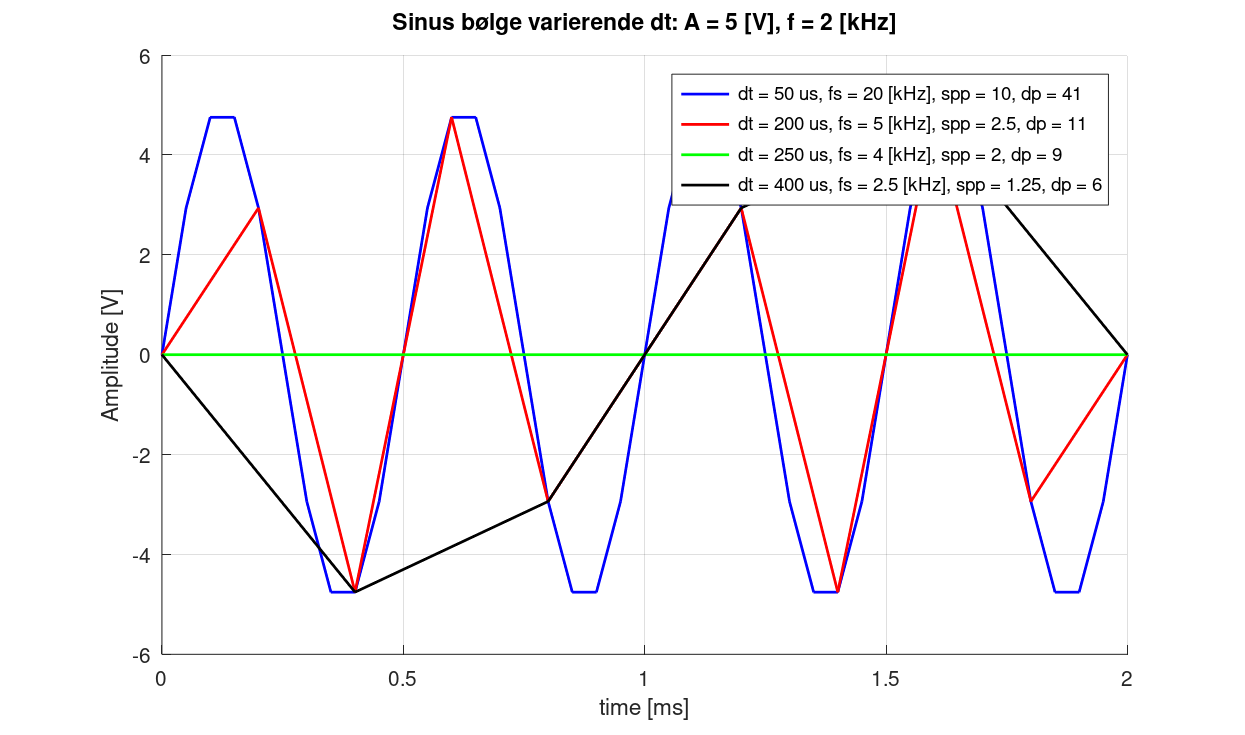
\includegraphics[width=0.9\textwidth]
    {Media/sammenlignei_dt_i_en_plot.png}
    \caption{Sammenligning av sinussignalet ved ulike steglengder.}
\end{figure}
\noindent De samme signalene vises også separat for å gjøre forskjellen mellom de ulike samplingsfrekvensene tydeligere.
\begin{figure}[H]
    \centering
    \includegraphics[width=1\textwidth]
    {fixedd_subplot_sammen_lignig_av_dt.png}
    \caption{De fire samplingsfrekvensene vist i separate diagrammer.}
\end{figure}
\noindent Ved $spp = 2$ er samplingsfrekvensen akkurat lik Nyquist-frekvensen. I dette tilfellet treffer samplingspunktene nullgjennomgangene til sinusbølgen, og signalet kan derfor ikke rekonstrueres fra de samplede verdiene. Dette viser hvorfor det i praksis er ønskelig med en samplingsfrekvens høyere enn $2f$.
\clearpage

\hypertarget{oppgave3}{}
\section*{Oppgave 3}
\addcontentsline{toc}{section}{Oppgave 3}

I denne oppgaven genereres firkantpulser og bitsekvenser i Octave.
For å gjøre dette er det laget egne funksjoner for generering av
signalene. Selve implementasjonen av funksjonene er lagt i
vedlegg A, mens denne delen viser hvordan funksjonene brukes og
resultatene de gir.
\begin{verbatim}
pkg load signal; # for å bruke square() funksjonen
\end{verbatim}

% --------------------------------------------------
\subsection*{a)}

For generering av firkantpulsen er funksjonen
\texttt{mySquareV1} laget. Funksjonen bruker signalets fase i
radianer og modulo $2\pi$ for å bestemme hvor i perioden hvert
sample befinner seg. \\[1em]
Det er også laget en alternativ funksjon, \texttt{mySquareV2},
som utfører tilsvarende generering direkte i tidsdomenet.
Implementasjonen av begge funksjonene finnes i vedlegg A.\\[1em]
Det brukes en fundamental frekvens på 10 kHz og 100 samples
per periode:
\begin{verbatim}
f0 = 10e3;
T = 1/f0;
fs = f0*100;

t_start = 0;
dt = 1/fs;
t_end = T*4-dt;

d_c = 50; # %
d_c2 = 20; # %

t = t_start:dt:t_end;
\end{verbatim}
Periodetiden er:
\[
    T = \frac{1}{f_0} = \frac{1}{10kHz} = 0.1\,\text{ms}
\]
Med 100 samples per periode blir samplingsfrekvensen:
\[
    f_s = 100f_0 = 1\,\text{MHz}
\]
Den egenlagde funksjonen brukes først til å generere en puls med
50 \% duty cycle. Deretter genereres en sentrert puls med
20 \% duty cycle:
\begin{verbatim}
[_, out_m] = mySquareV1(t, f0, d_c);
[_, out_m2] = mySquareV1(t, f0, d_c2, [0,1], 0, true);
\end{verbatim}
For å kontrollere resultatet sammenlignes signalene med Octaves
innebygde \texttt{square()}-funksjon:
\begin{verbatim}
out = square(t*2*pi*f0, d_c);

t_1 = T*(d_c2/100)/2;

out2 = square((t+t_1)*2*pi*f0, d_c2);
out2 = (out2 + 1)/2;
\end{verbatim}
Figuren viser at den egenlagde funksjonen gir samme firkantpulser
som \texttt{square()}-funksjonen.
\begin{figure}[H]
    \centering
    \includegraphics[width=1\textwidth]{oppgave3a.png}
    \caption{Sammenligning mellom den egenlagde
    \texttt{mySquareV1}-funksjonen og \texttt{square()} i Octave.}
\end{figure}

% --------------------------------------------------
\subsection*{b)}
For å generere en bitsekvens er funksjonen
\texttt{bitWaveGen} laget. Funksjonen mottar en bitvektor,
bittid, antall samples per bit og et eventuelt shift. Funksjonen bruker også hjelpefunksjonen
\texttt{addZerosOrOnes}. Implementasjonen av begge funksjonene finnes i vedlegg A.
Bitsekvensen som skal genereres er:
\[
[1,\ 0,\ 1,\ 0].
\]
Bittiden settes til 1 ms, med 100 samples per bit og et shift på 50 \%:
\begin{verbatim}
bits = [1,0,1,0];
T = 1e-3; # s
spp = 100; # sample per periode
sh = 50; # %

[t, out] = bitWaveGen(bits, T, spp, sh);
\end{verbatim}
Samplingsintervallet blir:
\[
dt = \frac{T}{100}
   = 10\,\mu\text{s}.
\]
Figuren under viser den resulterende bitsekvensen.
\begin{figure}[H]
    \centering
    \includegraphics[width=0.9\textwidth]{oppgave3b.png}
    \caption{Generert bitsekvens $[1,0,1,0]$ med
    100 samples per bit og 50 \% shift.}
\end{figure}

\clearpage

\hypertarget{Vedlegg A}{}
\section*{Vedlegg A}
\addcontentsline{toc}{section}{Vedlegg A}
\appendix

Dette vedlegget inneholder implementasjonen av de egenlagde
funksjonene som brukes i Oppgave 3.

% --------------------------------------------------
\subsection*{mySquareV1}

\begin{verbatim}
function [t, out] = mySquareV1(t, f0, d_c, ...
                               bds=[-1,1], pds=0, cent=false);
    #{
        Denne funksjonen genererer firkantpulsen ved å uttrykke
        signalets fase i radianer og bruke modulo 2*pi.

        t: tidsvektor
        f0: fundamental frekvens
        d_c: duty cycle
        bds:  grenser -> bds(1) = lav verdi, bds(2) = høy verdi.
        pds: antall perioder man ønsker: pds <= antall perioder det er i t
        cent: få en sentrert positiv puls omkring origo

        return verdier
        t:  pds=0 -> t_ut = t_in ellers er den tilpaset. [ms]
        out: resulterde verdier for y aksen (amplitude vektor).
    #}

    T = 1/f0;

    if pds != 0;
        t_stop = T*pds;
        idx = find(t >= t_stop, 1)-1;
        t = t(1:idx);
    end;

    d_c = d_c/100; # konverter til desimal
    rads = t*2*pi*f0; # konverter til radianer

    if cent;
        rads = t*2*pi*f0 + (2*pi*d_c)/2;
    end;

    pulse_end_rad = 2*pi*d_c; # når pulsen skal gå lavt igjen
    n_rad = mod(rads, 2*pi); # normaliser radianer til 0-2pi

    out = n_rad; 
    out(n_rad >= pulse_end_rad) = bds(1);
    out(n_rad < pulse_end_rad) = bds(2);

    t = t*1e3; # skaler til ms
end;
\end{verbatim}


% --------------------------------------------------
\subsection*{mySquareV2}

\begin{verbatim}
function [t, out] = mySquareV2(f0, d_c, spp, ...
                               bds=[-1,1], pds=5, sh=0);
    #{
        Denne funksjonen genererer firkantpulsen direkte i
        tidsdomenet ved å bruke modulo av periodetiden T.

        f0: fundamental frekvens
        d_c: duty cycle
        spp: samples per periode
        bds: grenser -> bds(1) = lav verdi, bds(2) = høy verdi.
        pds: antall perioder man ønsker
        shfit: sh i tid gitt i prosent -> t + T*(sh/100)

        return verdier
        t: resulterdne tidsavektor skalert til ms,
        out: resulterde verdier for y aksen (amplitude vektor).
    #}

    d_c = d_c/100; # konverter til desimal
    T = 1/f0; 
    dt = T/spp;
    pulse_end_time = T*d_c; # når pulsen skal gå lavt igjen i tid 

    t = 0:dt:(T*pds-dt);
    t_mod = mod(t + T*(sh/100), T); # normaliser (t + t_shift) til 0-T 

    out = t_mod;
    out(t_mod < pulse_end_time) = bds(2);
    out(t_mod >= pulse_end_time) = bds(1);

    t = t*1e3; # skaler til ms
end;
\end{verbatim}

% --------------------------------------------------
\subsection*{addZerosOrOnes}

\begin{verbatim}
function y = addZerosOrOnes(x, num);
    if x == 0;
        y = zeros(1, num);
    else
        y = ones(1, num);
    end;
end;
\end{verbatim}


% --------------------------------------------------
\subsection*{bitWaveGen}

\begin{verbatim}
function [t, out] = bitWaveGen(bits, T, spp, sh=0)
    #{
        bits: vektor med bits (1 og 0) som skal generere en puls
        T: bit tid (periode) i sekunder
        spp: samples per periode
        shift: sh i tid gitt i prosent -> t + T*(sh/100)

        return verdier
        t: resulterende tidsvektor skalert til ms,
        out: resulterende verdier for y aksen (amplitude vektor).
    #}

    dt = T/spp;
    pds = length(bits); # antall perioder
    sh_num = round(spp*(sh/100)); # antall som skal shiftes

    t = 0:dt:(T*pds-dt);
    out = [];

    first = bits(1); # bit som skal shiftes først

    for i=1:pds;

        if i == 1;
            out = [out, ...
                   addZerosOrOnes(bits(i), spp-sh_num)];
        else
            out = [out, ...
                   addZerosOrOnes(bits(i), spp)];
        end;
    end;

    # legg til shift rest på første bit tilbake i vektoren
    out = [out, addZerosOrOnes(first, sh_num)]; 

    t = t*1e3; # skaler til ms
end;
\end{verbatim}
\clearpage

\hypertarget{Vedlegg B}{}
\section*{Vedlegg B}
\addcontentsline{toc}{section}{Vedlegg B}
\appendix
GitHub repository for rapporten: \\
\indent Url: \href{https://github.com/Yonatan1717/SigB}{\textcolor{blue}{https://github.com/Yonatan1717/SigB}}\\
\indent Inneholder all kode og ploter i innleveringen.

\clearpage


\end{document}
